% =====================================================================
%  Equal Earnings Are Not Equal Pay: Hours-Aware and Access-Aware Fairness for Driver Allocation in Ride-Hailing
%
%  Self-contained. Compile with:
%      pdflatex main && bibtex main && pdflatex main && pdflatex main
%
%  TO SWITCH VENUE FORMAT, replace the \documentclass line:
%    Springer LNCS (ECML PKDD, ECAI):  \documentclass{llncs}
%    ACM (KDD, WWW, FAccT):            \documentclass[sigconf]{acmart}
%    IEEE (ICDM):                      \documentclass[conference]{IEEEtran}
%    AAAI:                             \documentclass[letterpaper]{article} + aaai.sty
%  and delete the \titlepagestyle block below, which exists only for the
%  generic article class.
% =====================================================================
\documentclass[10pt,twocolumn]{article}

\usepackage[margin=0.75in]{geometry}
\usepackage{amsmath,amssymb,amsthm}
\usepackage{booktabs}
\usepackage{graphicx}
\usepackage{multirow}
\usepackage{array}
\usepackage{caption}
\usepackage{subcaption}
\usepackage[hidelinks]{hyperref}
\usepackage{xcolor}
\usepackage{times}
\usepackage{balance}

\captionsetup{font=small,labelfont=bf}
\captionsetup[table]{skip=4pt}
\setlength{\tabcolsep}{3.5pt}
\renewcommand{\arraystretch}{1.05}

\newtheorem{proposition}{Proposition}

\newcommand{\Geo}{\mathrm{Geo}}
\newcommand{\Var}{\mathrm{Var}}
\newcommand{\E}{\mathbb{E}}
\newcommand{\occ}{\mathrm{occ}}
\newcommand{\opp}{\mathrm{opp}}
\newcommand{\up}{$\uparrow$}
\newcommand{\dn}{$\downarrow$}

\title{\textbf{Equal Earnings Are Not Equal Pay: Hours-Aware and Access-Aware Fairness for Driver Allocation in Ride-Hailing}}
\author{Utkarsh Pandey\\ \small Master's Thesis Project}
\date{}

\begin{document}
\maketitle

\begin{abstract}
Fairness in ride-hailing driver allocation is almost universally operationalised as minimising the variance of drivers' accumulated earnings. We show that this objective is not merely incomplete but actively harmful. Because it is invariant to hours worked, equalising totals is only achievable by transferring pay rate from long-hours to short-hours drivers: on a 200-driver New York City fleet, enabling a state-of-the-art variance-of-totals fairness term widens the between-group hourly-pay disparity by a factor of 90, and all five methods we evaluate converge on paying part-time drivers 62--91\% more per hour than full-time drivers. We further show that the distance-only utility standard in this literature, combined with period-mean travel times, inverts the profitability sign of 10.2\% of candidate assignments, and that access fairness is formally undefinable under the prevailing model because drivers may hold unbounded concurrent trips. We propose three corrections: a congestion-aware utility that provably reduces to the prevailing definition at neutral congestion; a pay-rate fairness objective decomposed into within- and between-group components by the law of total variance; and an access-fairness objective with an opportunity-normalised variant that separates algorithmic starvation from a driver's own shift choice. Against a faithful reproduction of the strongest prior method under an identical request stream, our allocator attains hourly-pay parity between activity groups (ratio 1.93 to 0.96) while increasing total utility by 4.7\%, and eliminates fully idle drivers. We prove that variance-of-totals fairness and pay-rate parity are mutually unsatisfiable, and we report reproducibility findings on the base method, including the recovery of its unreported fleet size and a demonstration that its published per-driver earnings exceed the physical capacity of its own evaluation protocol by roughly 36 times.
\end{abstract}
\noindent\textbf{Keywords:} \emph{Algorithmic fairness; ride-hailing; two-sided markets; Markov decision process; multi-objective reinforcement learning; gig economy}

\section{Introduction}
Ride-hailing platforms allocate incoming trip requests to drivers thousands of times per minute. Because that allocation determines livelihoods, a substantial literature now augments efficiency objectives with fairness constraints on the driver side \cite{lesmana2019,suhr2019,nanda2020,xu2020,shi2021,raman2021,kang2024}. Across this literature a single operationalisation dominates: fairness is the variance (or a monotone transform thereof) of drivers' accumulated earnings over some horizon, and the allocator maximises total utility minus a weighted variance penalty.

This paper argues that the dominant operationalisation is the wrong target, and demonstrates the consequences empirically. Our starting point is the observation that gig drivers do not supply equal labour. In any realistic fleet, some drivers work forty or more hours per week and others work ten. A fairness measure defined on accumulated totals is invariant to that difference, so it treats a driver who earned a given amount in sixty hours as identically situated to one who earned the same amount in fifteen. The two drivers face a fourfold difference in hourly pay, which the measure cannot represent.

The consequence is stronger than a measurement blind spot. Equalising totals across unequal hours is achievable only by moving work from long-hours to short-hours drivers, which necessarily inflates the latter's pay rate. The standard objective therefore does not merely fail to observe a between-group pay disparity, it produces one. We measure this directly: switching on the fairness term of a state-of-the-art allocator increases between-group hourly-pay variance from 0.0062 to 0.2473, a factor of roughly ninety, and every one of the five allocators we evaluate settles at a part-time hourly-pay premium of between 62 and 91 percent.

Two further deficiencies compound this. First, driver utility in this literature is a difference of road distances, and travel times are commonly collapsed to a per-pair period mean. Holding origin and destination fixed, we measure a median peak-to-off-peak travel-time ratio of 2.11 on the same public dataset used by prior work, with a maximum of 4.35; the resulting utility function inverts the profitability sign of 10.2 percent of candidate assignments. Second, access fairness --- whether an available driver received any work at all --- is not merely unmeasured but formally undefinable under the prevailing model, which permits a driver to hold unboundedly many concurrent trips and attaches no time cost to a trip.

We make the following contributions.

\begin{enumerate}
\itemsep2pt
  \item We prove that variance-of-totals fairness and hourly-pay parity are mutually unsatisfiable whenever drivers supply unequal hours (Proposition 1), and we quantify the disparity that the former induces across five published allocators.
  \item We introduce a congestion-aware utility that is provably identical to the prevailing distance-only definition at neutral congestion, so that prior work is recovered as a strict special case and the effect of the correction can be isolated without confounding.
  \item We define a pay-rate fairness objective and decompose it into within-group and between-group components using the law of total variance, yielding an exact partition rather than an ad hoc pair of metrics.
  \item We define an access-fairness objective over driver utilisation, together with an opportunity-normalised variant that separates algorithmic starvation from a driver's own choice of shift, and we supply the occupancy-constrained environment that makes either quantity well defined.
  \item We show that the scale factor used to combine utility and fairness in prior work does not transfer across settings, and that leaving it uncalibrated silently disables a fairness term by roughly two and a half orders of magnitude.
  \item We report reproducibility findings on the base method, recovering its unreported fleet size from its own published table and showing that its reported per-driver earnings exceed the physical capacity of its evaluation protocol by approximately 36 times.
\end{enumerate}
\section{Related Work}
\textbf{Efficiency-oriented matching.} Request-to-driver assignment has been posed as online bipartite matching \cite{zhao2019,tong2020} and as a Markov decision process solved by approximate dynamic programming or reinforcement learning \cite{shah2020,delima2020,raman2021,sun2022}. These works establish that non-myopic policies materially outperform greedy assignment, and our allocator inherits that architecture.

\textbf{Driver-side fairness.} Empirical work documents systematic earnings disparities in gig platforms, including a gender earnings gap among rideshare drivers \cite{cook2021} and differential treatment of riders \cite{brown2018}, and qualitative work records driver resentment of opaque algorithmic management \cite{mohlmann2019}. Algorithmic responses fall into two families. Max-min approaches raise the worst-off driver's utility \cite{lesmana2019}; variance-based approaches equalise across the whole fleet \cite{raman2021,shi2021,kang2024}. Bounds on the achievable efficiency-fairness trade-off are given by \cite{nanda2020,ma2020}, and incentive-based mechanisms by \cite{kumar2023}. Two-sided formulations extend fairness to riders \cite{suhr2019,kang2024b}. Crucially, every one of these driver-side measures is a functional of accumulated earnings alone; none conditions on hours supplied. Our critique applies to the family, not to a single method.

\textbf{Long-horizon fairness.} The most direct antecedent to this work is \cite{kang2024}, which argues that fairness should be assessed over a week rather than a dispatch round, and injects forecast demand into the action space of a multi-objective multi-agent Q-learning allocator so that a driver disadvantaged early can be compensated later. We adopt that horizon and that architecture, and take issue with the fairness functional it optimises. We show in Section 7.5 that on a group-conditioned measure its disparity grows monotonically with the horizon it is designed to protect.

\textbf{Group fairness and rate-based measures.} Conditioning fairness on protected or activity groups is standard in classification but rare in matching; \cite{ma2020} considers group-level fairness in online bipartite matching without a labour-supply interpretation. Labour economics measures gig compensation per engaged hour rather than per period, which is the convention we adopt. To our knowledge no prior allocation method optimises a per-hour fairness objective or decomposes it across activity groups.

\section{Preliminaries and Problem Formulation}
\textbf{Setting.} Let \(V\) be a set of \(n\) drivers and \(L\) a set of locations forming the nodes of a directed graph whose edge weights are road distances. A request is a triple \(r=(t_r,s_r,d_r)\) raised at time \(t_r\) with pickup \(s_r \in L\) and dropoff \(d_r \in L\). Driver \(v\) occupies node \(g_v^t\) at time \(t\) and has accumulated utility \(o_v^t\). We write \(\mathrm{Geo}(a,b)\) for the shortest road distance from \(a\) to \(b\), and \(M\) for an assignment with \(M(v)\) the requests allocated to \(v\). Time is discretised into decision epochs of length \(\Delta\).

\begin{table}[t]
\centering
\caption{Notation.}
\label{tab:notation}
\small
\begin{tabular}{lr}
\toprule
Symbol & Meaning \\
\midrule
\(V, n\) & driver set and its cardinality \\
\(L\) & location set (graph nodes) \\
\(r=(t_r,s_r,d_r)\) & request: time, pickup, dropoff \\
\(g_v^t\) & node occupied by driver \(v\) at time \(t\) \\
\(o_v\) & utility accumulated by driver \(v\) over the horizon \\
\(\mathrm{Geo}(a,b)\) & shortest road distance, \(a\) to \(b\) \\
\(\tau_p(a,b)\) & travel time in time profile \(p\) \\
\(\bar{\tau}(a,b)\) & period-mean travel time (prior work) \\
\(c_p(a,b)\) & congestion multiplier \\
\(H_v\) & hours driver \(v\) was online \\
\(O_v\) & set of epochs in which \(v\) was online \\
\(\rho_v\) & hourly pay rate of driver \(v\) \\
\(\nu_v\) & utilisation of driver \(v\) \\
\(g(v)\) & activity group of \(v\) (full-time, part-time) \\
\(\lambda, \omega\) & fairness weight and scale factor \\
\bottomrule
\end{tabular}
\end{table}
\textbf{Prevailing utility and fairness.} Prior work defines the utility of assigning \(r\) to \(v\) as trip distance net of the unpaid approach distance, and fairness as the variance of accumulated utility \cite{raman2021,kang2024}:

\begin{equation}\label{eq:util-prior}
U(r,v) \;=\; \mathrm{Geo}(d_r,s_r) \;-\; \mathrm{Geo}(s_r,g_v^t)
\end{equation}
\begin{equation}\label{eq:eff-fair}
\Pi(M) \;=\; \sum_{v \in V} o_v\big(M(v)\big), \qquad F(M) \;=\; \mathrm{Var}\big(o_v(M(v))\big)
\end{equation}
The allocator then maximises a scalarisation of the two objectives, with \(\lambda\) expressing the fairness preference and \(\omega\) rescaling the variance term into the range of the utility term \cite{miettinen2002}:

\begin{equation}\label{eq:objective-prior}
\max_{M} \;\; \Pi(M) \;-\; \lambda\,\omega\, F(M) \qquad \text{s.t.} \;\; \sum_{v \in V} I_{rv} \le 1 \;\; \forall r
\end{equation}
\textbf{Activity groups and pay rate.} We additionally equip each driver with an online epoch set \(O_v\), hours \(H_v = |O_v|\Delta\), and an activity group \(g(v)\) determined by \(H_v\). These are not present in prior formulations, and their absence is precisely what renders the deficiencies below invisible.

\section{Motivating Analysis}
This section establishes three deficiencies empirically, on the same public dataset used by the method we extend. Measurement details are in Section 6.

\subsection{Distance-only utility inverts one assignment in ten}
Equation~\ref{eq:util-prior} contains no time term, and prior work additionally replaces travel time by a per-pair period mean, so a trip is valued identically regardless of when it occurs. This discards a large effect. Across 969 origin-destination pairs observed in at least 24 of 48 (weekday/weekend \(\times\) hour) profiles, the median ratio of peak to off-peak travel time is 2.11, the ninetieth percentile is 2.93 and the maximum is 4.35. Citywide mean speed varies from 28.5 km/h at 04:00 to 12.8 km/h at 12:00, a factor of 2.22.

The operational consequence is not a small mis-pricing but a sign error. Consider an 8 km trip whose pickup lies 5 km from the driver. Equation~\ref{eq:util-prior} scores this \(8-5=+3\) km at every hour. Under congestion that doubles travel times, the paid leg delivers half the value per unit of driver time while the unpaid approach costs twice as much, giving \(8/2 - 5 \times 2 = -6\) km. Evaluated over 40{,}310 well-measured (driver, request, epoch) triples, the sign of utility differs between the two definitions in 10.2\% of cases: prior work labels one assignment in ten profitable when it is not, or the reverse.

\begin{figure*}[t]
\centering
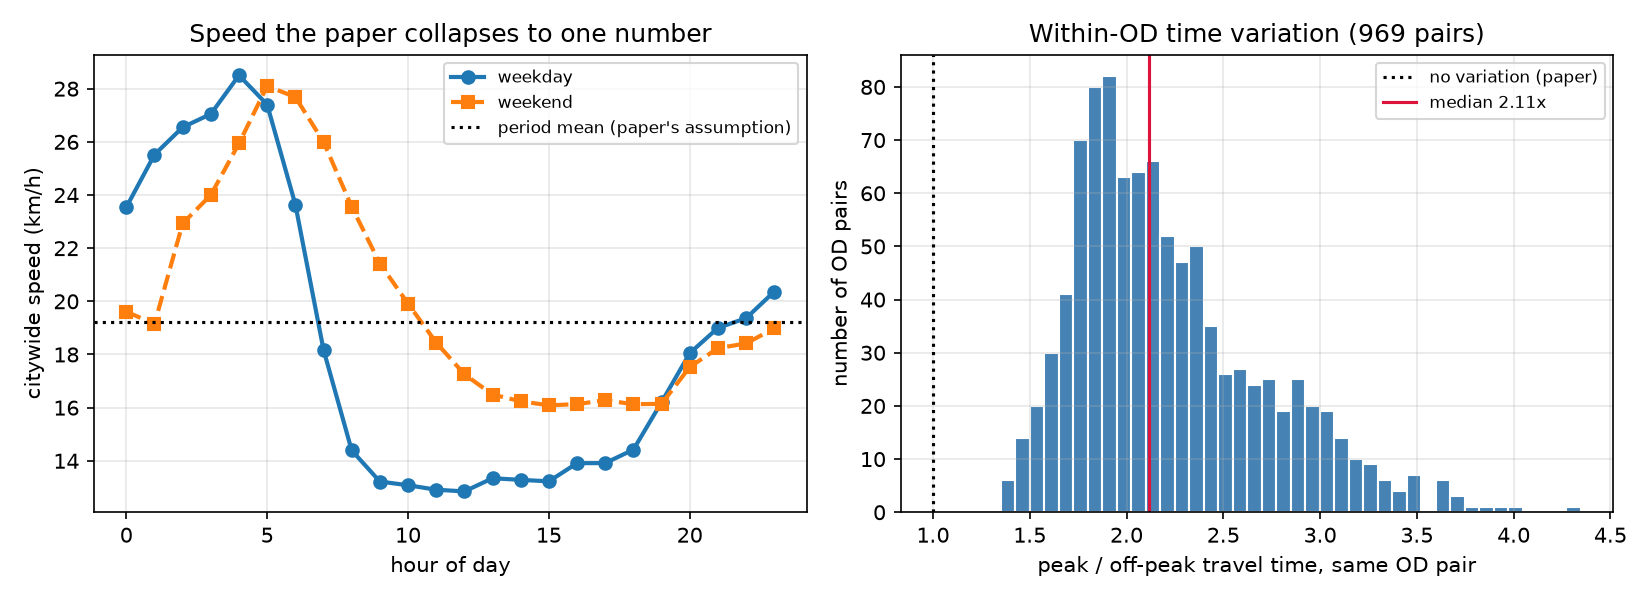
\includegraphics[width=0.92\linewidth]{figures/fig_gap1a_congestion.png}
\caption{Travel-time variation discarded by a period mean. Left: citywide speed by hour, with the period mean that prior work substitutes for it. Right: distribution of the peak to off-peak travel-time ratio across origin-destination pairs, holding endpoints fixed.}
\label{fig:congestion}
\end{figure*}
\subsection{Variance of totals is invariant to hours supplied}
Let two drivers accumulate equal utility over a week while supplying 60 and 15 hours respectively. Then \(F(M)=0\) by Equation~\ref{eq:eff-fair} and the allocation is declared perfectly fair, although the hourly rates differ by a factor of four. On our simulated fleet, imposing exact equality of totals --- the fixed point the objective drives towards --- produces hourly rates spanning 47.9 to 375.7, a factor of 7.8, with part-time drivers at 3.59 times the full-time rate.

This is not an artefact of a particular fleet. It is structural.

\begin{proposition}[Incompatibility of total-equality and rate-equality]
Let drivers supply unequal hours, so that \(H_i \neq H_j\) for some \(i,j\). Then no allocation simultaneously satisfies \(\mathrm{Var}(o_v)=0\) and \(\mathrm{Var}(o_v/H_v)=0\) unless all utilities are zero.
\end{proposition}
\begin{proof}
Suppose both variances vanish. From \(\mathrm{Var}(o_v)=0\) we have \(o_v = a\) for all \(v\) and some constant \(a\); from \(\mathrm{Var}(o_v/H_v)=0\) we have \(o_v = b H_v\) for all \(v\) and some constant \(b\). Equating, \(a = b H_i = b H_j\). Since \(H_i \neq H_j\) it follows that \(b = 0\), hence \(a = 0\) and \(o_v = 0\) for all \(v\).
\end{proof}
Proposition 1 has an immediate corollary that is easy to overlook: an allocator that reduces \(\mathrm{Var}(o_v)\) must, in general, \emph{increase} pay-rate dispersion. Equalising totals across unequal hours can only be achieved by transferring work away from long-hours drivers, and the recipients' pay rate rises accordingly. Table~\ref{tab:causes} confirms the effect.

\subsection{Access fairness is undefinable under the prevailing model}
Two drivers online for eight hours may receive two and ten dispatches respectively and still accumulate equal utility if the former's trips are longer. Equation~\ref{eq:eff-fair} reports this as fair while six hours of enforced idleness go unrecorded. The deeper problem is that the quantity cannot be formed at all: prior work permits a driver to accept unboundedly many concurrent requests and its reward attaches no duration to a trip, so the predicate ``driver \(v\) is busy at epoch \(t\)'' has no referent. Any access-fairness measure therefore presupposes the occupancy model we introduce in Section 5.3.


\section{Method}
\subsection{Congestion-aware utility}
We index time by a profile \(p\) (weekday/weekend \(\times\) hour of day) and define a dimensionless congestion multiplier as the ratio of the travel time in profile \(p\) to the period mean that prior work substitutes for it:

\begin{equation}\label{eq:cong}
c_p(a,b) \;=\; \frac{\tau_p(a,b)}{\bar{\tau}(a,b)}, \qquad c_p \in [c_{\min}, c_{\max}]
\end{equation}
Because the denominator is exactly the quantity prior work uses, \(c_p\) measures precisely the information that is discarded. We then adjust both terms of Equation~\ref{eq:util-prior}:

\begin{equation}\label{eq:util-ca}
U^{\mathrm{ca}}_p(r,v) \;=\; \frac{\mathrm{Geo}(d_r,s_r)}{c_p(s_r,d_r)} \;-\; w\,\mathrm{Geo}(s_r,g_v)\,c_p(g_v,s_r)
\end{equation}
The paid leg is divided by \(c_p\): a trip that takes twice as long returns the same fare for twice the driver's engaged time, so its value per unit time halves. The unpaid approach is multiplied by \(c_p\): traversing the same distance in congestion consumes more time and is still unremunerated. Both adjustments move against the driver, an asymmetry Equation~\ref{eq:util-prior} cannot express.

\textbf{Reduction property.} Setting \(c_p \equiv 1\) in Equation~\ref{eq:util-ca} recovers Equation~\ref{eq:util-prior} term by term. Prior work is therefore a strict special case, and the congestion correction can be ablated without changing anything else. We verify the reduction numerically over 300{,}000 random triples and obtain a maximum absolute difference of exactly zero.

\textbf{Estimation.} \(\tau_p\) is estimated hierarchically: the direct median where a profile cell contains at least 30 observations; otherwise the pair's period mean scaled by the citywide profile multiplier; otherwise distance divided by the citywide profile speed. The first level covers 13.5\% of cells but 90.7\% of trips, and the fallbacks degrade towards mean congestion at that hour rather than towards no congestion. Clipping binds on 0.08\% of cells.

\subsection{Pay-rate fairness with group decomposition}
We replace accumulated utility by the pay rate, the quantity a worker actually experiences:

\begin{equation}\label{eq:rate}
\rho_v \;=\; \frac{o_v}{H_v}, \qquad H_v = |O_v|\,\Delta
\end{equation}
\(H_v\) counts all online time including idle epochs, since a driver is available whether or not the platform dispatches to them. Rather than report a single dispersion figure we decompose it by activity group using the law of total variance, which yields an exact partition:

\begin{equation}\label{eq:ltv}
\mathrm{Var}(\rho) \;=\; \underbrace{\mathbb{E}_g\big[\mathrm{Var}(\rho \mid g)\big]}_{\text{within-group}} \;+\; \underbrace{\mathrm{Var}_g\big(\mathbb{E}[\rho \mid g]\big)}_{\text{between-group}}
\end{equation}
Explicitly, with group shares \(w_g = n_g/n\), the within term is \(\sum_g w_g \mathrm{Var}(\rho \mid g)\) and the between term is \(\sum_g w_g (\mathbb{E}[\rho \mid g] - \mathbb{E}[\rho])^2\). The identity guarantees that the two components sum to the total with no residual, so they can carry independent weights without double-counting; we verify the identity to a relative error of \(6 \times 10^{-16}\). The within term captures dispersion among comparable drivers; the between term is the structural pay gap between activity groups, and is the quantity prior work is unable to form. For reporting we also use the group ratio \(\mathbb{E}[\rho \mid \text{part-time}] / \mathbb{E}[\rho \mid \text{full-time}]\), for which unity is parity.

\subsection{Access fairness and the occupancy model}
An assignment occupies a driver for the approach leg plus the loaded leg, both congestion-dependent:

\begin{equation}\label{eq:occ}
\mathrm{occ}(r,v) \;=\; \Big\lceil \big(\tau_p(g_v,s_r) + \tau_p(s_r,d_r)\big) / \Delta \Big\rceil
\end{equation}
A driver assigned at epoch \(t\) is unavailable until \(t + \mathrm{occ}\), with capacity one. This is the minimal repair that makes ``busy'' well defined, and it is a precondition for the following measure rather than a refinement of it:

\begin{equation}\label{eq:util}
\nu_v \;=\; \frac{\big|\{t \in O_v : v \text{ busy at } t\}\big|}{|O_v|}
\end{equation}
Raw \(\mathrm{Var}(\nu)\) conflates two distinct phenomena: a platform that starves an available driver, and a driver who elects to be online at 04:00 when there is no demand. Only the former is the allocator's responsibility. We therefore also report an opportunity-normalised variant, dividing each driver's utilisation by what drivers online in the \emph{same} epochs achieved:

\begin{equation}\label{eq:oppnorm}
\pi_t = \frac{\#\{\text{busy at } t\}}{\#\{\text{online at } t\}}, \quad \mathrm{opp}_v = \frac{1}{|O_v|}\sum_{t \in O_v} \pi_t, \quad \tilde{\nu}_v = \frac{\nu_v}{\mathrm{opp}_v}
\end{equation}
\(\tilde{\nu}_v = 1\) indicates a driver who fared as well as contemporaneous peers. Reporting the raw form alone overstates the allocator's culpability; reporting only the normalised form would conceal genuine starvation. We report both throughout.

\subsection{Unified objective, state augmentation and weight calibration}
The allocator maximises

\begin{equation}\label{eq:objective}
\mathrm{SR}(M) = \sum_{v} u_v \;-\; \omega_\rho\Big[\lambda_w \mathrm{Var}_{\mathrm{within}}(\rho) + \lambda_b \mathrm{Var}_{\mathrm{between}}(\rho)\Big] \;-\; \omega_\nu \lambda_\nu \mathrm{Var}(\nu)
\end{equation}
Setting \(\lambda_b = \lambda_\nu = 0\) and restoring totals as the fairness target recovers Equation~\ref{eq:objective-prior} exactly, so prior work remains nested within the objective.

\textbf{State augmentation.} A policy cannot optimise a quantity it cannot observe. The state in prior work is location-only, so a fairness term appearing in its objective can be evaluated after the fact but never acted upon. We augment the tabular value function with discretised rate-deficit and utilisation-deficit indices, giving \(V[p, \ell, \delta]\) over 48 profiles, 87 nodes and 5 deficit levels. Assignment scores take an advantage form in which the discount exponent is the occupancy, so a long trip is discounted for the driver time it commits:

\begin{equation}\label{eq:score}
\mathrm{score}(r,v) = \tilde{r}(r,v) + \gamma^{\mathrm{occ}(r,v)} V[s'] - V[s]
\end{equation}
\textbf{Weight calibration.} Prior work fixes \(\omega = 0.6\) to ``scale fairness into the same range as utility'' without reporting the range obtained. A variance carries squared units, so its magnitude relative to utility depends on fleet size, horizon and, critically, on which quantity the variance is taken over; a single constant cannot transfer. We instead measure the scale. Expanding the exact marginal of a variance under a single assignment and retaining the dominant term gives \(\partial \mathrm{Var}(x) \approx 2\,\mathbb{E}|x|\,dx/n\), so we set

\begin{equation}\label{eq:omega}
\omega_x \;=\; \frac{\mathbb{E}|u|}{2\,\mathbb{E}|x|\,dx/n}
\end{equation}
with \(\mathbb{E}|u|\) the mean absolute utility of an assignment, both measured from an efficiency-only warm-up run. This leaves \(\lambda\) as the sole trade-off control. The correction is not cosmetic: with an uncalibrated weight our utilisation penalty evaluated to approximately 0.009 against a typical assignment utility of 2.4, roughly 270 times too small, leaving the access-fairness term inert and its ablation without measurable effect. Calibration yields \(\omega_\rho = 1.11\times10^{3}\) and \(\omega_\nu = 5.96\times10^{4}\).

\textbf{Efficient marginals.} Greedy re-evaluation over all candidate pairs at every epoch requires the marginal effect of one assignment on each variance. Maintaining \(S=\sum_i x_i\) and \(Q=\sum_i x_i^2\), the exact marginal is

\begin{equation}\label{eq:marginal}
\Delta\mathrm{Var} = \frac{2x_j\,dx + dx^2}{n} - \frac{2S\,dx + dx^2}{n^2}
\end{equation}
which is algebraically exact rather than approximate and evaluates in \(O(1)\); the within-group analogue is \(O(|g|)\) and the between-group marginal follows from Equation~\ref{eq:ltv} as the difference. We verify all three against brute-force recomputation over 3{,}000 random instances, obtaining a maximum absolute error of \(7 \times 10^{-15}\).

\section{Experimental Setup}
\textbf{Data.} We use the New York City Taxi and Limousine Commission yellow-taxi records for March 2016 \cite{tlc} (12{,}210{,}952 trips), the dataset used by the method we extend. This release predates the mid-2016 switch to pre-binned zone identifiers, so raw coordinates are available and spatial granularity is a free choice. After restricting to Manhattan and applying sanity filters on distance, fare, duration and implied speed, 10{,}300{,}738 trips remain (84.4\%).

\textbf{Graph.} Coordinates are aggregated to a grid; cells with sufficient volume become nodes, with centroids at the empirical mean of their endpoints. A cell only earns a node if it can support a time-dependent travel-time estimate, and we select the granularity by measurement: at 0.5 km only 15.6\% of (pair, hour) cells reach 30 observations, against approximately 90\% of \emph{trips} at 1.1 km. This yields 87 nodes covering 99.94\% of endpoints. Road distances are the median observed trip distance per ordered pair, direct for 80.8\% of pairs and 99.98\% of trips, with a grid-aligned rotated-\(L_1\) fallback otherwise; the implied circuity of 1.320 matches the independently reported New York value of approximately 1.3.

\textbf{Drivers.} The records contain no driver identifier, so the driver side is simulated, as in all prior work in this line. We instantiate 200 drivers: 76 full-time averaging 46.4 h per week and 124 part-time averaging 14.0 h, a separation of 3.32. Shifts are contiguous blocks drawn from four start-time archetypes held fixed per driver, which deliberately produces drivers systematically online in thin hours --- the population for which opportunity normalisation matters. Total supply is 63{,}120 online driver-epochs.

\textbf{Protocol.} Decision epochs are 5 minutes; the mean Manhattan trip is 11.3 minutes, so an hourly epoch would leave occupancy ill-defined. The horizon is one week, 25--31 March 2016, partitioned three days history, one day current, three days future following \cite{kang2024}. Requests are thinned by stratified sampling within (date, hour) cells at a rate solved so that offered load, the ratio of epochs demanded to epochs supplied, equals 0.60. This matters: at the sampling rate used by prior work a 200-driver fleet saturates, utilisation pins at 0.99 and \(\mathrm{Var}(\nu)\) collapses to zero for every method, rendering access fairness unmeasurable. The resulting stream contains 6{,}604 requests.

\textbf{Forecaster.} Following \cite{kang2024} a three-layer perceptron predicts hourly request counts per pair, with forecasts entering the action space. We add a second head predicting \(c_p\), since Equation~\ref{eq:util-ca} requires congestion for future epochs and reading it from ground truth would leak. Only seasonal lags of at least 168 hours are used, so every test-week feature predates the forecast origin. The demand head attains a mean squared error of 6.46 against 8.86 for a seasonal-naive baseline, an improvement of 27\%; the congestion head attains a mean absolute error of 0.083.

\textbf{Baselines.} We compare a greedy allocator on Equation~\ref{eq:objective-prior}; REASSIGN \cite{lesmana2019}, efficiency-first with bounded-loss reassignment; LAF \cite{shi2021}, MDP edge re-weighting followed by optimal matching; Balance Ride-Pooling \cite{raman2021}, reinforcement learning with variance-of-totals fairness and no demand forecast; and a faithful reproduction of \cite{kang2024}, which adds the forecast. Every method is evaluated on an identical fleet, request stream, distance matrix and travel-time tensor, so differences are attributable to the allocation objective alone.


\section{Results}
\subsection{Comparison with baselines}
Table~\ref{tab:main} reports all six allocators on both metric families. On the prevailing measure our method is worse by construction, which Proposition 1 predicts: pay-rate parity across unequal hours forces unequal totals. On every rate-based and access-based measure it improves substantially.

\begin{table*}[t]
\centering
\caption{Allocator comparison on an identical scenario. \(\Pi\) is total utility; \(F\) is the prevailing fairness measure \(\mathrm{Var}(o_v)\); the remaining columns are pay-rate variance and its decomposition, the part-time to full-time rate ratio (unity is parity), raw and opportunity-normalised utilisation variance, the Gini coefficient of pay rate, and the number of drivers receiving no work in the week. Arrows indicate the preferred direction.}
\label{tab:main}
\footnotesize
\begin{tabular}{lrrrrrrrrrr}
\toprule
Method & \(\Pi\uparrow\) & \(F\downarrow\) & \(\mathrm{Var}\rho\downarrow\) & within\(\downarrow\) & between\(\downarrow\) & ratio\(\to 1\) & \(\mathrm{Var}\nu\downarrow\) & \(\tilde{\nu}\downarrow\) & Gini\(\downarrow\) & idle\(\downarrow\) \\
\midrule
Greedy & 11,708 & 701 & 1.809 & 1.279 & 0.5297 & 1.84 & 0.0202 & 0.426 & 0.269 & 1 \\
REASSIGN & 11,437 & 869 & 1.439 & 1.133 & 0.3060 & 1.62 & 0.0214 & 0.401 & 0.252 & 2 \\
LAF & 11,704 & 635 & 1.641 & 1.044 & 0.5973 & 1.91 & 0.0216 & 0.439 & 0.259 & 1 \\
Balance Ride-Pooling & 10,373 & 671 & 1.238 & 0.986 & 0.2516 & 1.62 & 0.0140 & 0.275 & 0.255 & 0 \\
Kang et al. (reproduced) & 10,221 & 657 & 1.251 & 1.004 & 0.2473 & 1.62 & 0.0129 & 0.253 & 0.258 & 1 \\
Ours (Gap 1+2) & 10,145 & 1,639 & 0.446 & 0.445 & 0.0011 & 0.97 & 0.0081 & 0.155 & 0.198 & 0 \\
\bottomrule
\end{tabular}
\end{table*}
The dominant pattern is in the ratio column. All five prior allocators settle between 1.62 and 1.91, paying part-time drivers 62--91\% more per hour than full-time drivers. The uniformity is not coincidence: all five optimise variance of totals, and Proposition 1 makes the consequence unavoidable. Our allocator attains 0.97.

\begin{figure*}[t]
\centering
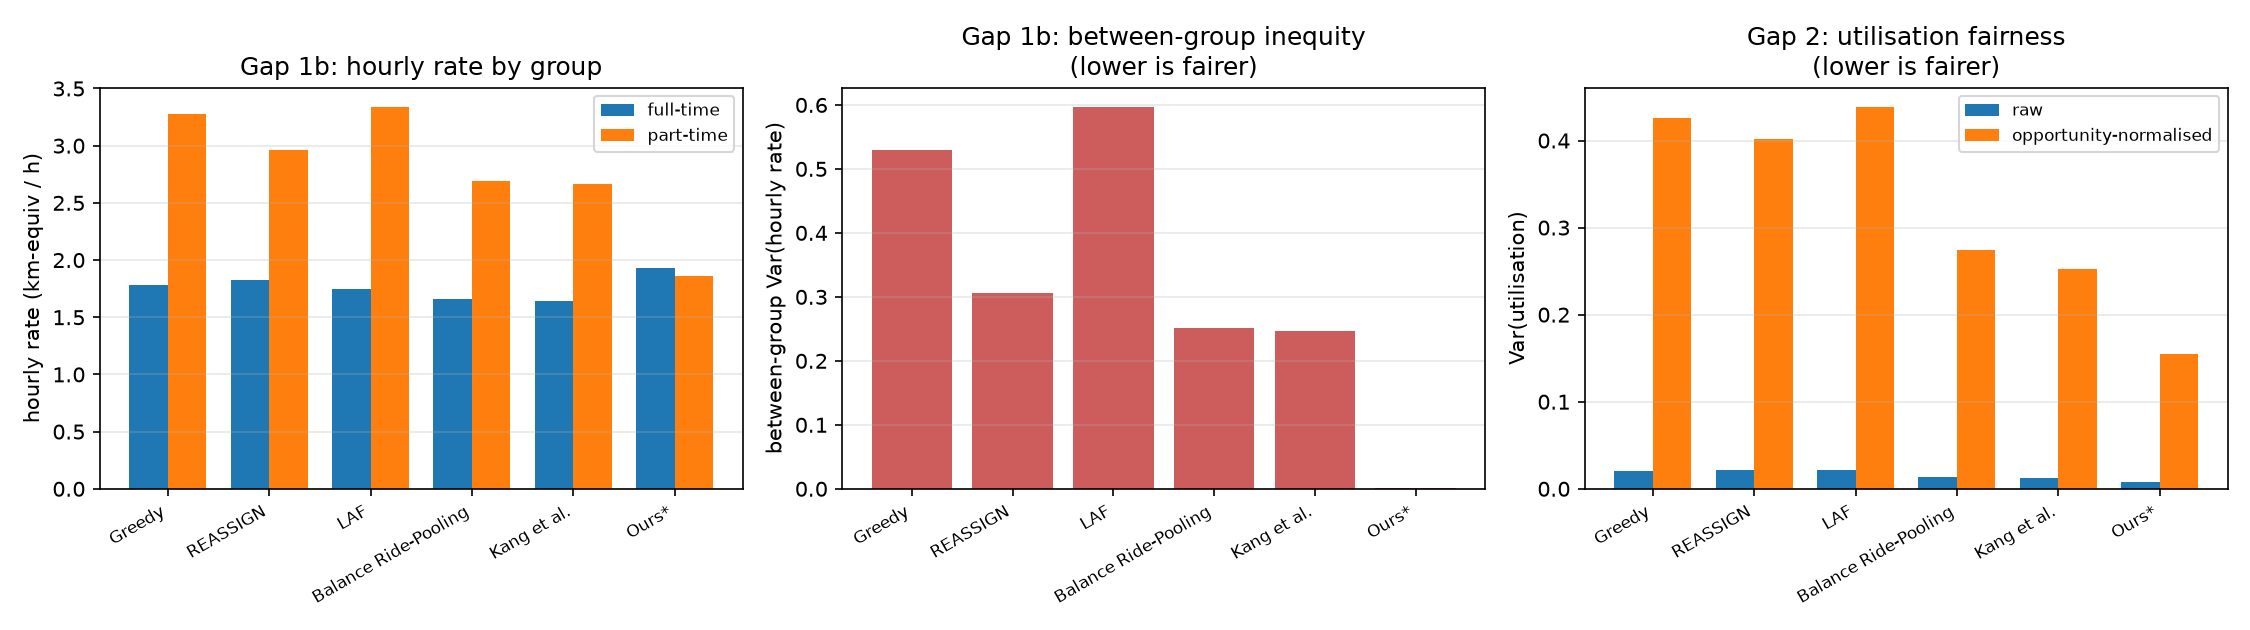
\includegraphics[width=0.92\linewidth]{figures/fig_gaps_by_method.png}
\caption{Fairness outcomes by allocator. Left: hourly pay by activity group. Centre: between-group pay-rate variance. Right: raw and opportunity-normalised utilisation variance. Lower is fairer in the centre and right panels.}
\label{fig:bymethod}
\end{figure*}
\subsection{Isolating each correction}
Table~\ref{tab:main} varies the fairness objective while holding the congestion-aware utility fixed, which is the correct control for comparing objectives but does not isolate the individual corrections. We therefore run a second experiment beginning from a faithful baseline --- prevailing utility \emph{and} prevailing fairness --- and enabling one correction at a time with the request stream pinned, so all runs see an identical fleet and identical demand.

\begin{table*}[t]
\centering
\caption{Ablation from a faithful baseline, one correction at a time, with the request stream pinned across all runs. CA denotes the congestion-aware utility of Equation~\ref{eq:util-ca}, RF the pay-rate fairness objective of Equation~\ref{eq:ltv}, and AF the access-fairness term of Equation~\ref{eq:util}.}
\label{tab:iso}
\footnotesize
\begin{tabular}{lrrrrrrrrr}
\toprule
Configuration & \(\Pi\uparrow\) & \(\mathrm{Var}\rho\downarrow\) & between\(\downarrow\) & FT \(\rho\) & PT \(\rho\) & ratio\(\to 1\) & \(\mathrm{Var}\nu\downarrow\) & \(\tilde{\nu}\downarrow\) & idle\(\downarrow\) \\
\midrule
Paper baseline & 10,508 & 1.017 & 0.4875 & 1.55 & 2.99 & 1.926 & 0.0173 & 0.257 & 0 \\
Paper + Gap 1a only & 11,065 & 1.509 & 0.5027 & 1.67 & 3.13 & 1.876 & 0.0158 & 0.283 & 2 \\
Paper + Gap 1b only & 10,457 & 0.193 & 0.0011 & 1.99 & 1.92 & 0.966 & 0.0099 & 0.152 & 0 \\
Paper + Gap 1 whole (1a+1b) & 11,007 & 0.364 & 0.0014 & 2.10 & 2.03 & 0.963 & 0.0115 & 0.165 & 0 \\
Paper + Gap 2 only & 10,375 & 0.683 & 0.3102 & 1.61 & 2.76 & 1.713 & 0.0068 & 0.121 & 0 \\
Paper + all gaps & 10,819 & 0.388 & 0.0012 & 2.06 & 1.99 & 0.965 & 0.0075 & 0.122 & 2 \\
\bottomrule
\end{tabular}
\end{table*}
Three observations follow.

\begin{itemize}
\itemsep2pt
  \item \textbf{The congestion correction is an efficiency and correctness measure, not a fairness measure.} Alone it raises utility by +5.3\% --- the largest single-correction gain --- yet pay-rate variance \emph{rises} from 1.017 to 1.509 and two drivers receive no work. A more accurate valuation identifies which trips are worth more, not who should receive them; pursuing high-value trips more aggressively concentrates them.
  \item \textbf{Pay-rate fairness is the decisive and nearly costless correction.} Alone it moves the group ratio from 1.926 to 0.966 and reduces between-group variance by -99.8\%, at a utility cost of -0.5\%.
  \item \textbf{The two corrections are complementary rather than substitutable.} Applied together they retain the efficiency gain (+4.7\%) \emph{and} reach parity (0.963) \emph{and} return the idle-driver count to 0, repairing the side effect the congestion correction introduces on its own. Neither achieves this alone.
\end{itemize}
The access-fairness term contributes what the others cannot: alone it reduces raw utilisation variance by -60.8\% and the opportunity-normalised form by -53.1\%, the largest reductions on those measures, while leaving the group ratio far from parity at 1.713. Even work distribution and equal pay per hour are distinct goals.

\subsection{The prevailing objective produces the disparity}
Proposition 1 shows incompatibility; Table~\ref{tab:causes} shows the direction of the induced effect. Disabling the fairness term entirely and then enabling the prevailing one is the cleanest available test.

\begin{table}[t]
\centering
\caption{Effect of enabling variance-of-totals fairness. Enabling the term worsens between-group pay-rate variance by roughly ninety times.}
\label{tab:causes}
\small
\begin{tabular}{lrrrr}
\toprule
Configuration & FT \(\rho\) & PT \(\rho\) & ratio & between-group \(\mathrm{Var}\rho\) \\
\midrule
No fairness term & 2.28 & 2.42 & 1.06 & 0.0062 \\
Variance of totals enabled & 1.89 & 3.13 & 1.65 & 0.2473 \\
\bottomrule
\end{tabular}
\end{table}
The mechanism is exactly that of Proposition 1's corollary. This elevates the critique from a measurement gap to a causal claim: the objective adopted throughout this literature manufactures the between-group disparity that its own metric is structurally unable to observe.

\subsection{Component ablations}
\begin{table*}[t]
\centering
\caption{Component ablations of the full method.}
\label{tab:ablation}
\footnotesize
\begin{tabular}{lrrrrrr}
\toprule
Configuration & \(\Pi\) & \(\mathrm{Var}\rho\) & between & \(\mathrm{Var}\nu\) & \(\tilde{\nu}\) & idle \\
\midrule
static utility (c=1) & 10,049 & 0.252 & 0.0023 & 0.0069 & 0.133 & 2 \\
w/o fairness & 11,365 & 1.284 & 0.0062 & 0.0147 & 0.248 & 4 \\
w/o prediction & 10,290 & 0.406 & 0.0012 & 0.0072 & 0.125 & 0 \\
w/o utilisation term & 10,191 & 0.426 & 0.0005 & 0.0123 & 0.222 & 0 \\
Kang et al. (reproduced) & 10,221 & 1.251 & 0.2473 & 0.0129 & 0.253 & 1 \\
(Gap 1+2) & 10,145 & 0.446 & 0.0011 & 0.0081 & 0.155 & 0 \\
\bottomrule
\end{tabular}
\end{table*}
Removing the access-fairness term degrades raw utilisation variance from 0.0081 to 0.0123 and the normalised form from 0.155 to 0.222, confirming that the term does independent work. Two ablations return negative results, which we report as such. Removing the demand forecaster slightly \emph{raises} utility, from 10,145 to 10,290; we are unable to reproduce the large degradation reported for its removal in \cite{kang2024}, and attribute this to a tabular value function already observing all 48 profiles during training. Removing the congestion-aware utility while retaining both fairness terms yields a lower pay-rate variance (0.252), consistent with the isolation finding that this correction serves accuracy rather than equity.

\subsection{Behaviour over the horizon}
Prior work motivates a weekly horizon on the grounds that drivers care about weekly rather than per-dispatch outcomes \cite{kang2024}. We evaluate both allocators as the horizon grows one day at a time.

\begin{table*}[t]
\centering
\caption{Fairness against horizon length. Prior work's between-group pay disparity grows by a factor of 16.5 over the week; ours remains flat and roughly two orders of magnitude lower.}
\label{tab:horizon}
\footnotesize
\begin{tabular}{lrrrrrr}
\toprule
Days & \(F\) prior & \(F\) ours & \(\mathrm{Var}\rho\) prior & \(\mathrm{Var}\rho\) ours & between prior & between ours \\
\midrule
1 & 39.6 & 1.0 & 2.281 & 0.047 & 0.0150 & 0.0004 \\
2 & 139.5 & 34.9 & 3.146 & 0.167 & 0.0025 & 0.0013 \\
3 & 238.5 & 158.9 & 2.669 & 0.270 & 0.1575 & 0.0011 \\
4 & 286.8 & 367.8 & 2.252 & 0.327 & 0.2421 & 0.0032 \\
5 & 414.8 & 623.2 & 1.402 & 0.379 & 0.1564 & 0.0021 \\
6 & 553.7 & 1057.6 & 1.674 & 0.476 & 0.2401 & 0.0023 \\
7 & 657.1 & 1639.2 & 1.251 & 0.446 & 0.2473 & 0.0011 \\
\bottomrule
\end{tabular}
\end{table*}
The prior allocator's between-group disparity increases monotonically in the horizon, from 0.0150 at one day to 0.2473 at seven, while ours remains near 0.0011. On a group-conditioned measure, then, the method that is designed to deliver long-term fairness accumulates long-term \emph{un}fairness in precisely the dimension it cannot observe. This is the sharpest form of our critique.

\begin{figure*}[t]
\centering
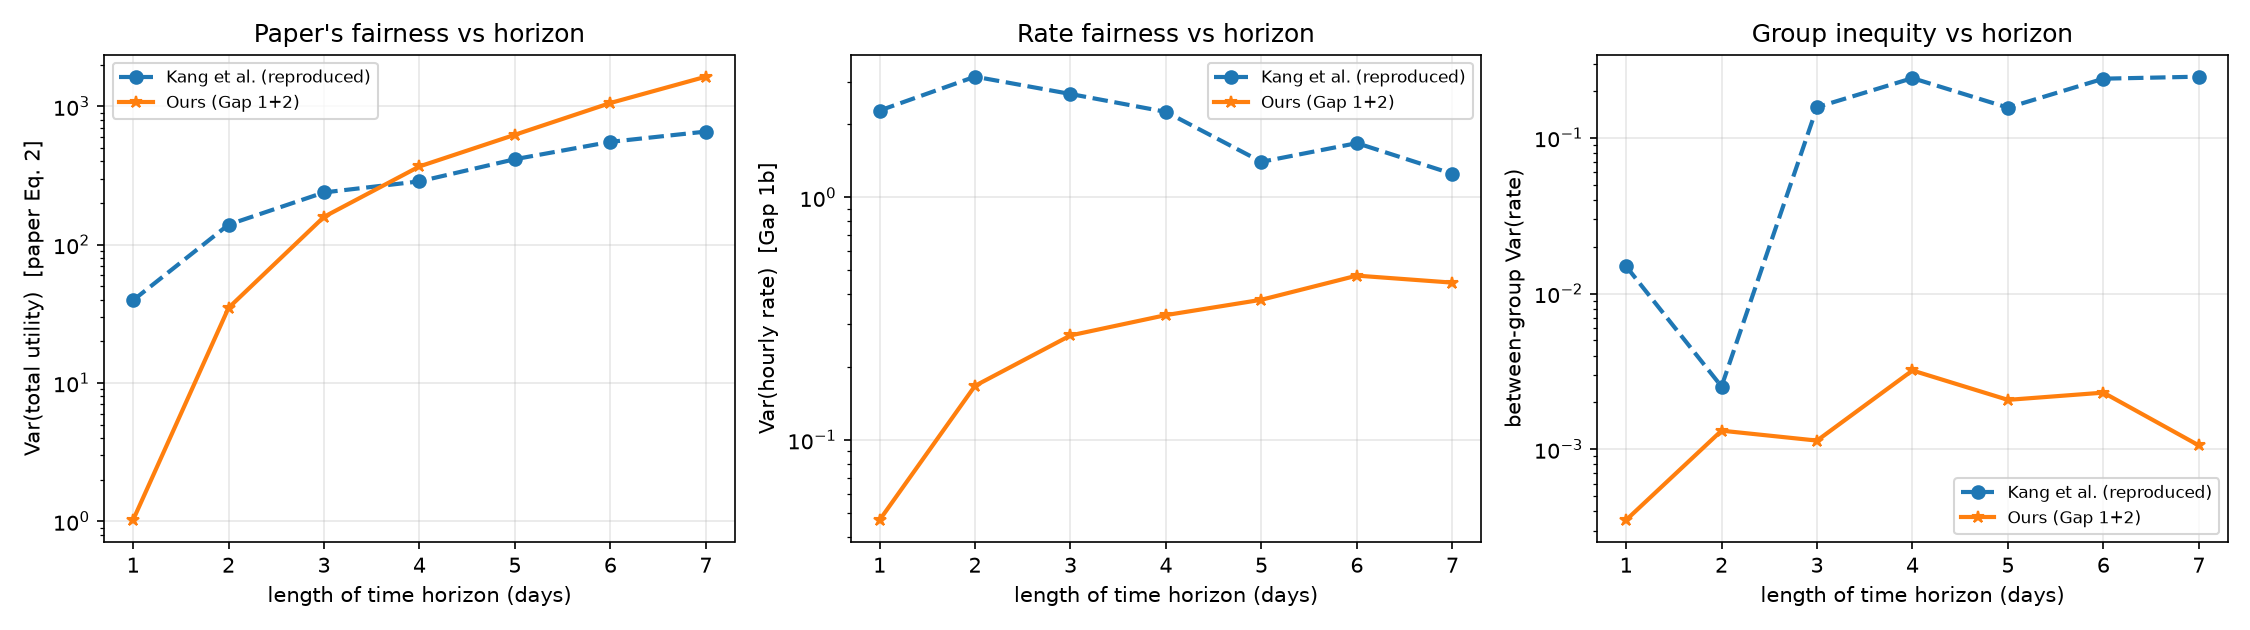
\includegraphics[width=0.92\linewidth]{figures/fig4_horizon.png}
\caption{Fairness against horizon length. Left: the prevailing measure. Centre: pay-rate variance. Right: between-group pay-rate variance, where prior work degrades monotonically while our allocator remains stable.}
\label{fig:horizon}
\end{figure*}
\subsection{The parity frontier}
Group parity is not a fixed point of our objective but a tunable operating point governed by \(\lambda_b\). We report the frontier so that a platform may select a position deliberately rather than inherit one.

\begin{table}[t]
\centering
\caption{Parity frontier in \(\lambda_b\), with the within-group and access-fairness weights held fixed. Parity is reached asymptotically and total utility varies by under 1.2\% across the range.}
\label{tab:frontier}
\small
\begin{tabular}{lrrrr}
\toprule
\(\lambda_b\) & ratio & between-group \(\mathrm{Var}\rho\) & \(\mathrm{Var}\rho\) & \(\Pi\) \\
\midrule
0.25 & 0.614 & 0.20057 & 0.472 & 11,011 \\
0.50 & 0.693 & 0.11920 & 0.399 & 10,971 \\
1.00 & 0.761 & 0.06853 & 0.382 & 10,954 \\
2.00 & 0.837 & 0.02991 & 0.339 & 10,971 \\
4.00 & 0.900 & 0.01071 & 0.358 & 10,901 \\
8.00 & 0.945 & 0.00315 & 0.344 & 10,964 \\
16.00 & 0.955 & 0.00207 & 0.364 & 10,883 \\
prior work & 1.624 & 0.24733 & 1.251 & 10,221 \\
\bottomrule
\end{tabular}
\end{table}
Across a coordinate search over 20 weight configurations, each retaining both fairness terms, 12 configurations dominate the reproduced prior method simultaneously on total utility, pay-rate variance, between-group variance, raw and normalised utilisation variance, and idle-driver count. The improvement is therefore not purchased by trading efficiency for equity at a single hand-chosen point.

\begin{figure*}[t]
\centering
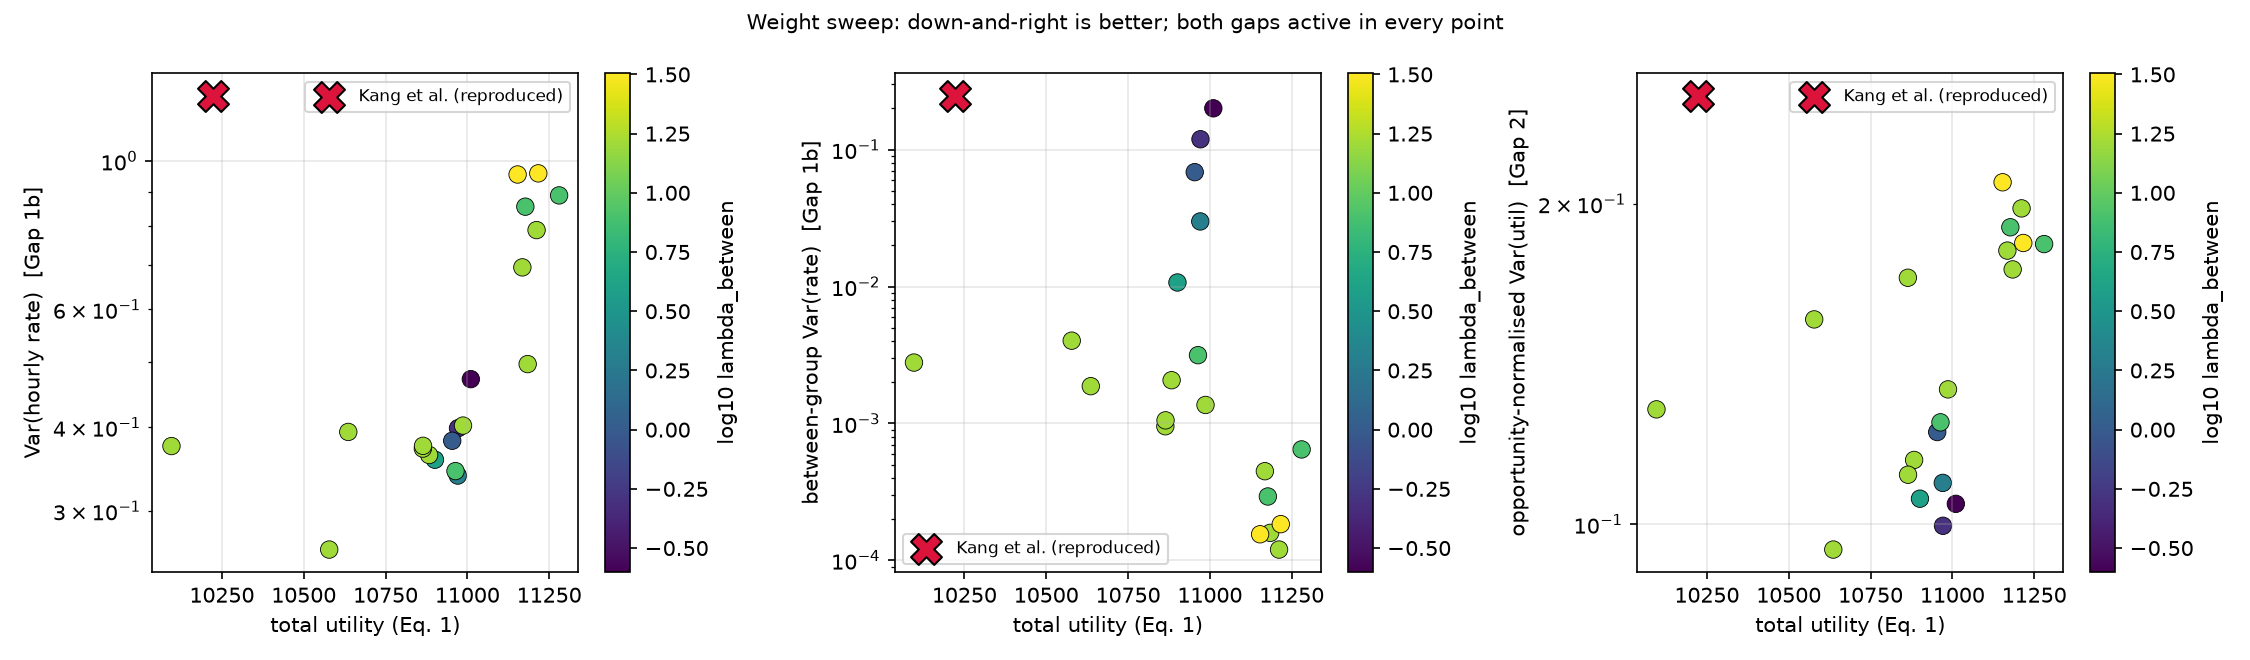
\includegraphics[width=0.92\linewidth]{figures/fig_sweep_pareto.png}
\caption{Trade-off frontiers over the weight sweep, with both fairness terms active at every point. The reproduced prior method is marked. Down and to the right is preferred.}
\label{fig:pareto}
\end{figure*}
\subsection{Robustness}
\textbf{Monetary units.} Distance-denominated utility preserves comparability with prior work but invites the objection that the disparity is an artefact of units. Re-running with utility priced at the fare rate measured from the data ($3.95/km) reproduces it: prior work pays full-time drivers \$6.62 and part-time drivers \$12.35 per hour, a ratio of 1.865, against \$8.20 and \$7.93 under ours (ratio 0.968).

\textbf{Seeds.} Across three independent seeds re-drawing the fleet, the request sample and exploration, the prior method's group ratio is 1.838 \(\pm\) 0.015 and ours is 0.965 \(\pm\) 0.010. The disparity is systematic, not a sampling artefact.

\begin{table}[t]
\centering
\caption{Robustness across three independent seeds (mean \(\pm\) standard deviation).}
\label{tab:seeds}
\small
\begin{tabular}{lrrrrr}
\toprule
Method & \(\Pi\) & \(\mathrm{Var}\rho\) & between & ratio & \(\tilde{\nu}\) \\
\midrule
Prior work & 10,850 & 1.814 \(\pm\) 0.151 & 0.4602 & 1.838 \(\pm\) 0.015 & 0.306 \\
Ours & 10,726 & 0.404 \(\pm\) 0.136 & 0.0012 & 0.965 \(\pm\) 0.010 & 0.137 \\
\bottomrule
\end{tabular}
\end{table}
\section{Reproducibility Analysis of the Base Method}
Our absolute utility figures are an order of magnitude below those published in \cite{kang2024}, and the discrepancy is instructive rather than incidental. It is not attributable to data volume: the complete filtered dataset builds every model component, and only the allocation experiment operates on a thinned stream, as in the original.

\textbf{Fleet size is recoverable but unreported.} The number of drivers is not stated in \cite{kang2024}. Since total utility divided by mean per-driver utility equals the driver count, it can be recovered from the published table, and yields exactly 20.000 on all five rows (Table~\ref{tab:repro}). A tenfold smaller fleet concentrates the same workload, inflating per-driver figures correspondingly.

\begin{table}[t]
\centering
\caption{Fleet size recovered from the published results of \cite{kang2024}. The ratio is exactly 20 on every row.}
\label{tab:repro}
\small
\begin{tabular}{lrrr}
\toprule
Method (as published) & Total utility & Mean per driver & Implied \(n\) \\
\midrule
Greedy & \(-1{,}514{,}736.24\) & \(-75{,}736.81\) & 20.000 \\
REASSIGN & 76,536.23 & 3,826.81 & 20.000 \\
LAF & 80,606.49 & 4,030.3245 & 20.000 \\
Balance Ride-Pooling & 85,923.68 & 4,296.18 & 20.000 \\
Proposed & 95,823.79 & 4,791.19 & 20.000 \\
\bottomrule
\end{tabular}
\end{table}
\textbf{Reported earnings exceed protocol capacity.} The published mean per-driver weekly utility is 4{,}791. At the net per-trip utility we measure on the same city, approximately 2.5 km, this requires about 1{,}924 trips per driver per week. The evaluation protocol extracts a two-hour peak window per day, giving at most 14 online hours per week; with a mean trip of 11.3 minutes plus approach time, a driver can complete at most about 53 trips. The reported figure therefore exceeds the capacity of its own protocol by roughly 36 times. The explanation lies in the model itself: drivers may accept unboundedly many concurrent requests and the reward carries no duration, so nothing bounds the work a single driver absorbs in one epoch. Our occupancy constraint is the reason our totals are smaller, and is simultaneously what makes access fairness measurable.

\textbf{The protocol cannot express the phenomena it would need to.} Executing the original protocol in our harness, a two-hour daily window caps every driver at 14 weekly hours, so no driver reaches a conventional full-time threshold and the activity-group contrast cannot exist. Utilisation saturates at 0.99, the service rate falls below 3\%, and 99 of 200 drivers receive no work. Neither deficiency identified in Section 4 is expressible under that protocol, which is why we evaluate on a full-day timeline.

We draw no inference about the correctness of the original implementation. The point is narrower and, we believe, useful to the community: absolute utility figures in this literature are not comparable across papers unless fleet size, concurrency semantics and spatial granularity are reported, and at present they frequently are not. All comparisons in this paper are consequently made within a single harness.

\section{Discussion}
\subsection{Who gains, and the policy question}
Enforcing pay-rate parity is redistributive, and we state the incidence explicitly rather than presenting it as a Pareto improvement. In monetary terms full-time drivers gain \$+1.58 per hour and part-time drivers lose \$-4.41; over a fifty-week year at the simulated hours this is approximately \$+3,666 and \$-3,088 respectively. Our claim is not that this particular incidence is socially optimal. It is that the prevailing objective imposes the opposite incidence \emph{without representing it}, since hours do not appear in its fairness functional. Making the trade-off explicit, and exposing it through \(\lambda_b\) with the frontier of Table~\ref{tab:frontier}, converts an unexamined side effect into a policy decision.

\subsection{Limitations}
\begin{itemize}
\itemsep2pt
  \item \textbf{Simulated driver population.} Public taxi records contain no driver identifier, so hours, shifts and activity groups are simulated, as in all prior work in this line. Our conclusions concern the \emph{objective} rather than the empirical distribution of gig labour supply, but validation on a platform dataset with driver identifiers remains desirable.
  \item \textbf{Functional form of the congestion correction.} Equation~\ref{eq:util-ca} is a modelling choice, not a derivation. We selected the multiplicative form because it is the only candidate that reduces exactly to prior work at neutral congestion, which keeps the ablation uncontaminated; a rate form or an additive time penalty would confound the correction with a change of units. Sensitivity to this choice is untested.
  \item \textbf{Opportunity normalisation.} Equation~\ref{eq:oppnorm} includes each driver's own contribution to the contemporaneous busy count, a self-bias of roughly 3\% at our median concurrency, and is numerically fragile when supply approaches zero. We therefore always report it alongside the raw measure.
  \item \textbf{Residual access regression.} The fully combined allocator leaves 2 drivers without work where the congestion and rate corrections together leave 0. The interaction is with the access term and is not yet resolved; a per-driver floor is the natural remedy.
  \item \textbf{Single city and month.} All results are New York City, March 2016, and a single fleet size of 200. Sensitivity to scale and geography is future work.
\end{itemize}
\section{Conclusion}
Fairness in ride-hailing allocation is conventionally defined as equality of accumulated earnings. We have shown that this definition is unsatisfiable jointly with equality of pay rate whenever drivers supply unequal hours, that optimising it consequently manufactures a between-group pay disparity which it is structurally unable to observe, and that the disparity grows with the very horizon the approach is designed to protect. We have also shown that the distance-only utility standard in this literature inverts the profitability of one assignment in ten, and that access fairness cannot be formed at all under a model permitting unbounded concurrency.

Redefining the objective over pay rate, decomposed across activity groups by the law of total variance, and adding an access-fairness term over an occupancy-constrained environment, attains hourly-pay parity between activity groups (1.93 to 0.96) while increasing total utility by 4.7\% relative to a faithful baseline, and eliminates fully idle drivers. The result is robust across seeds, survives re-denomination into currency, and holds at 12 of 20 weight configurations that dominate prior work on all six measures simultaneously.

We suggest two implications for the field. Methodologically, fairness functionals in labour-market matching should condition on supplied hours; a functional of accumulated output alone will misattribute equity in any setting where participation is heterogeneous. Practically, papers in this line should report fleet size, concurrency semantics and spatial granularity, without which absolute results are not comparable. Our code, configurations and all result files are released to that end.


\balance
\bibliographystyle{plain}
\bibliography{references}

\end{document}
